%% This is file `elsarticle-template-1-num.tex',
%%
%% Copyright 2009 Elsevier Ltd
%%
%% This file is part of the 'Elsarticle Bundle'.
%% ---------------------------------------------
%%
%% It may be distributed under the conditions of the LaTeX Project Public
%% License, either version 1.2 of this license or (at your option) any
%% later version.  The latest version of this license is in
%%    http://www.latex-project.org/lppl.txt
%% and version 1.2 or later is part of all distributions of LaTeX
%% version 1999/12/01 or later.
%%
%% Template article for Elsevier's document class `elsarticle'
%% with numbered style bibliographic references
%%
%% $Id: elsarticle-template-1-num.tex 149 2009-10-08 05:01:15Z rishi $
%% $URL: http://lenova.river-valley.com/svn/elsbst/trunk/elsarticle-template-1-num.tex $
%%
\documentclass[preprint,12pt]{elsarticle}

\usepackage{isotope} % \isotope command

%% Use the option review to obtain double line spacing
%% \documentclass[preprint,review,12pt]{elsarticle}

%% Use the options 1p,twocolumn; 3p; 3p,twocolumn; 5p; or 5p,twocolumn
%% for a journal layout:
%% \documentclass[final,1p,times]{elsarticle}
%% \documentclass[final,1p,times,twocolumn]{elsarticle}
%% \documentclass[final,3p,times]{elsarticle}
%% \documentclass[final,3p,times,twocolumn]{elsarticle}
%% \documentclass[final,5p,times]{elsarticle}
%% \documentclass[final,5p,times,twocolumn]{elsarticle}

%% The graphicx package provides the includegraphics command.
\usepackage{graphicx}
%% The amssymb package provides various useful mathematical symbols
\usepackage{amssymb}
%% The amsthm package provides extended theorem environments
%% \usepackage{amsthm}

%% The lineno packages adds line numbers. Start line numbering with
%% \begin{linenumbers}, end it with \end{linenumbers}. Or switch it on
%% for the whole article with \linenumbers after \end{frontmatter}.
\usepackage{lineno}

%% natbib.sty is loaded by default. However, natbib options can be
%% provided with \biboptions{...} command. Following options are
%% valid:

%%   round  -  round parentheses are used (default)
%%   square -  square brackets are used   [option]
%%   curly  -  curly braces are used      {option}
%%   angle  -  angle brackets are used    <option>
%%   semicolon  -  multiple citations separated by semi-colon
%%   colon  - same as semicolon, an earlier confusion
%%   comma  -  separated by comma
%%   numbers-  selects numerical citations
%%   super  -  numerical citations as superscripts
%%   sort   -  sorts multiple citations according to order in ref. list
%%   sort&compress   -  like sort, but also compresses numerical citations
%%   compress - compresses without sorting
%%
%% \biboptions{comma,round}

% \biboptions{}

\journal{Journal Name}

\begin{document}

\begin{frontmatter}

%% Title, authors and addresses

\title{A Stroboscopic Approach to Neutrino Oscillometry}

%% use the tnoteref command within \title for footnotes;
%% use the tnotetext command for the associated footnote;
%% use the fnref command within \author or \address for footnotes;
%% use the fntext command for the associated footnote;
%% use the corref command within \author for corresponding author footnotes;
%% use the cortext command for the associated footnote;
%% use the ead command for the email address,
%% and the form \ead[url] for the home page:
%%
%% \title{Title\tnoteref{label1}}
%% \tnotetext[label1]{}
%% \author{Name\corref{cor1}\fnref{label2}}
%% \ead{email address}
%% \ead[url]{home page}
%% \fntext[label2]{}
%% \cortext[cor1]{}
%% \address{Address\fnref{label3}}
%% \fntext[label3]{}


%% use optional labels to link authors explicitly to addresses:
%% \author[label1,label2]{<author name>}
%% \address[label1]{<address>}
%% \address[label2]{<address>}

\author{J. Doe}

\address{University of Amazements; Anywhere, USA}

\begin{abstract}
%% Text of abstract
New advances in technology have enabled the detailed resolution of substructure in neutrino beams. A number of notable analyses by the MINOS and MiniBooNE collaborations have already looked at detailed features in the arrival time of neutrino bunches. Pushing that capability to even finer time scales, it becomes possible to select different neutrino energy spectra based on their arrival time of the neutrinos relative to the bunch time. Later neutrinos within the bunch correspond to slower and therefore lower energy parent hadrons. We show that this effect could be resolved by detectors with order 100 psec vertex time resolution, but is limited by the current bunch size of the protons impinging on the target. Efforts to shorten the width of neutrino bunches to below 500 psec would greatly enhance this effect. The ability to reconstruct neutrino oscillations, selecting for different neutrino energy spectra would greatly control against flux and energy reconstruction uncertainties. Off-axis experiments can only sample a small slice of the angular flux spectrum. A stroboscopic approach would be analogous to sampling multiple off-axis angles within a single detector, and could be applied equally to both near and far detectors in an oscillation experiment. This motivates the continued development of time-of-flight capabilities in neutrino detectors, as well as further optimiztion of neutrino beams. 


\end{abstract}



\begin{keyword}
Timing \sep Timing
%% keywords here, in the form: keyword \sep keyword

%% MSC codes here, in the form: \MSC code \sep code
%% or \MSC[2008] code \sep code (2000 is the default)

\end{keyword}

\end{frontmatter}

%%
%% Start line numbering here if you want
%%
\linenumbers

%% main text
\section{Introduction}
\label{sec:intro}

The discovery of Charge-parity (CP) violation in the neutrino sector hinges on high precision, increasingly systematics-dominated measurements of neutrino oscillation parameters. The dominant systematic uncertainties

The wide span of energies in neutrino beams stems from the wide range of energies among the parent hadrons and is limited by the ability to cool and focus those beams. One handle for understanding.

Another handle for understanding and selecting different energy spectra within a neutrino beam exploits the differing velocities of the parent hadrons. Lower energy pions and kaons travel more slowly, especially as they approach sub-relativistic energies. As a consequence, lower energy neutrinos start further behind the rest of the bunch and selecting later arriving neutrinos would provide an increasingly pure low-energy subset of the overall flux.

The idea of using timing to resolve beam structure has a long history. Efforts to detect dark matter have relied on time-of-flight differences between dark matter particles and neutrinos. Timing has successfully been employed to identify a pure sample of stopped kaons and pions in neutrino beams. Several notable efforts have utilized bunch timing to place limits on neutrino velocity. MINOS, in particular, noted interesting kinematic relationships within the beam time. The MiniBooNE collaboration even explored the idea of using timing to select on the neutrino energy spectrum. However, efforts to select different energy spectra on the basis of beam timing have been largely overlooked due to two considerations: (1) Limited time resolutions of the detectors themselves were insufficient to see the O(100) psec effect, and (2) the $\sim$900 psec spread of the proton bunch impinging on the target washes out most of the effect.

In this paper, we revisit the idea of using beam timing to select different energy components of the neutrino flux. We show that existing precision timing technology is capable of resolving O(100) psec time-of-flight differences in neutrinos arrival times. {\it More importantly, we argue that feasible modifications to existing proton beams could superimpose a hyper-fine bunch structure on the protons, providing short enough bunches, spaced widely enough to fully exploit the energy spreading effect.}

The power of this technique stems from the fact that, in contrast to off-axis measurements, the different neutrino energy spectra can be selected within the same detector. Moreover, these timing relationships can be applied in near and far detector alike.

\begin{figure}[t]
	\begin{center}
           	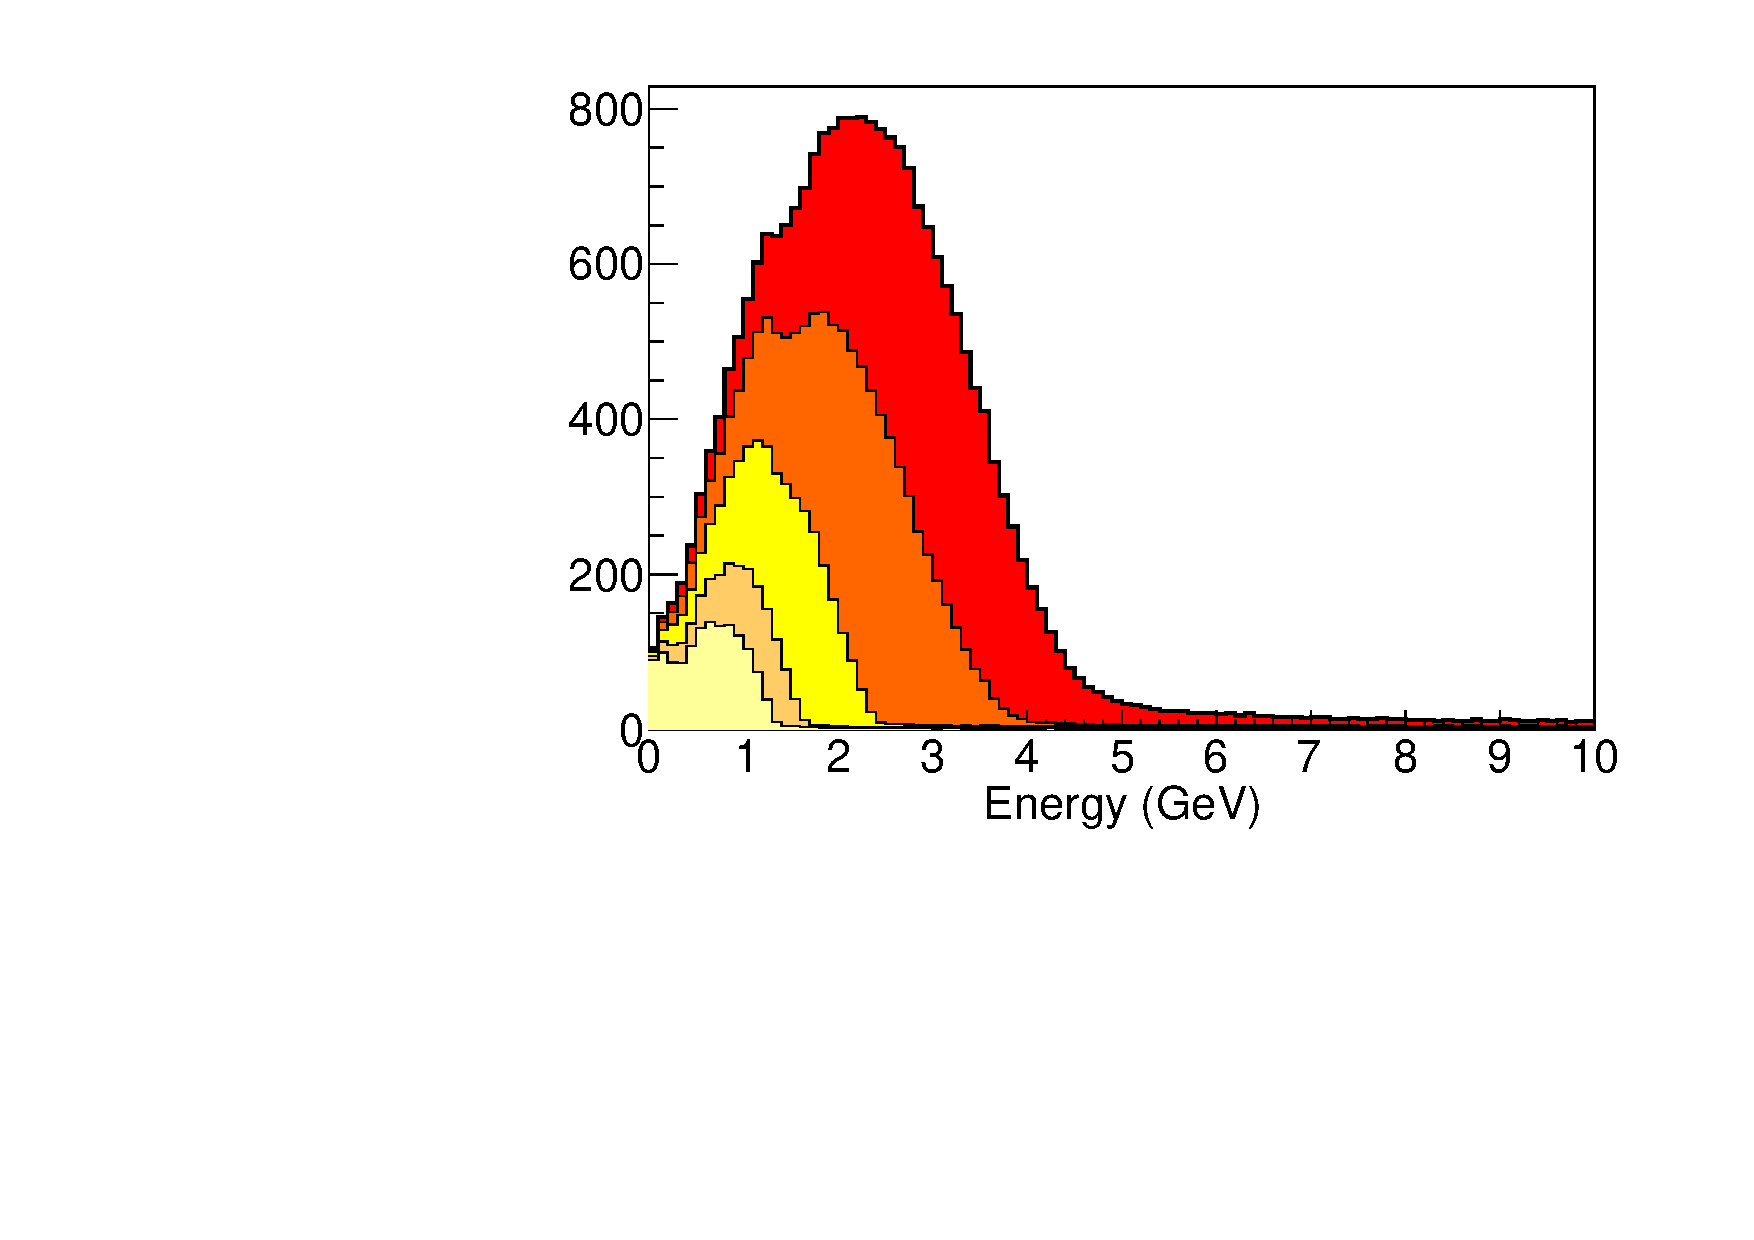
\includegraphics[width=0.45 \linewidth]{Figures/10.10.18_LBNFtiming/DUNEbeam_truetimingB.pdf}
	\end{center}
	\caption{The DUNE forward horn current flux (red), with the fluxes corresponding to increasingly later time-cuts on the bunch time, assuming no time spread of the protons on target: 250 psec after the start of the neutrino bunch (orange), 500 psec after (yellow), 750 psec (dark beige), 1 nsec (light beige).}
		\label{fig:anniedetector}
\end{figure}


\section{The Mechanism}

A brief discussion of the relationship between pion energy and speed

\begin{figure}[t]
	\begin{center}
           	\begin{tabular}{c c}	
           	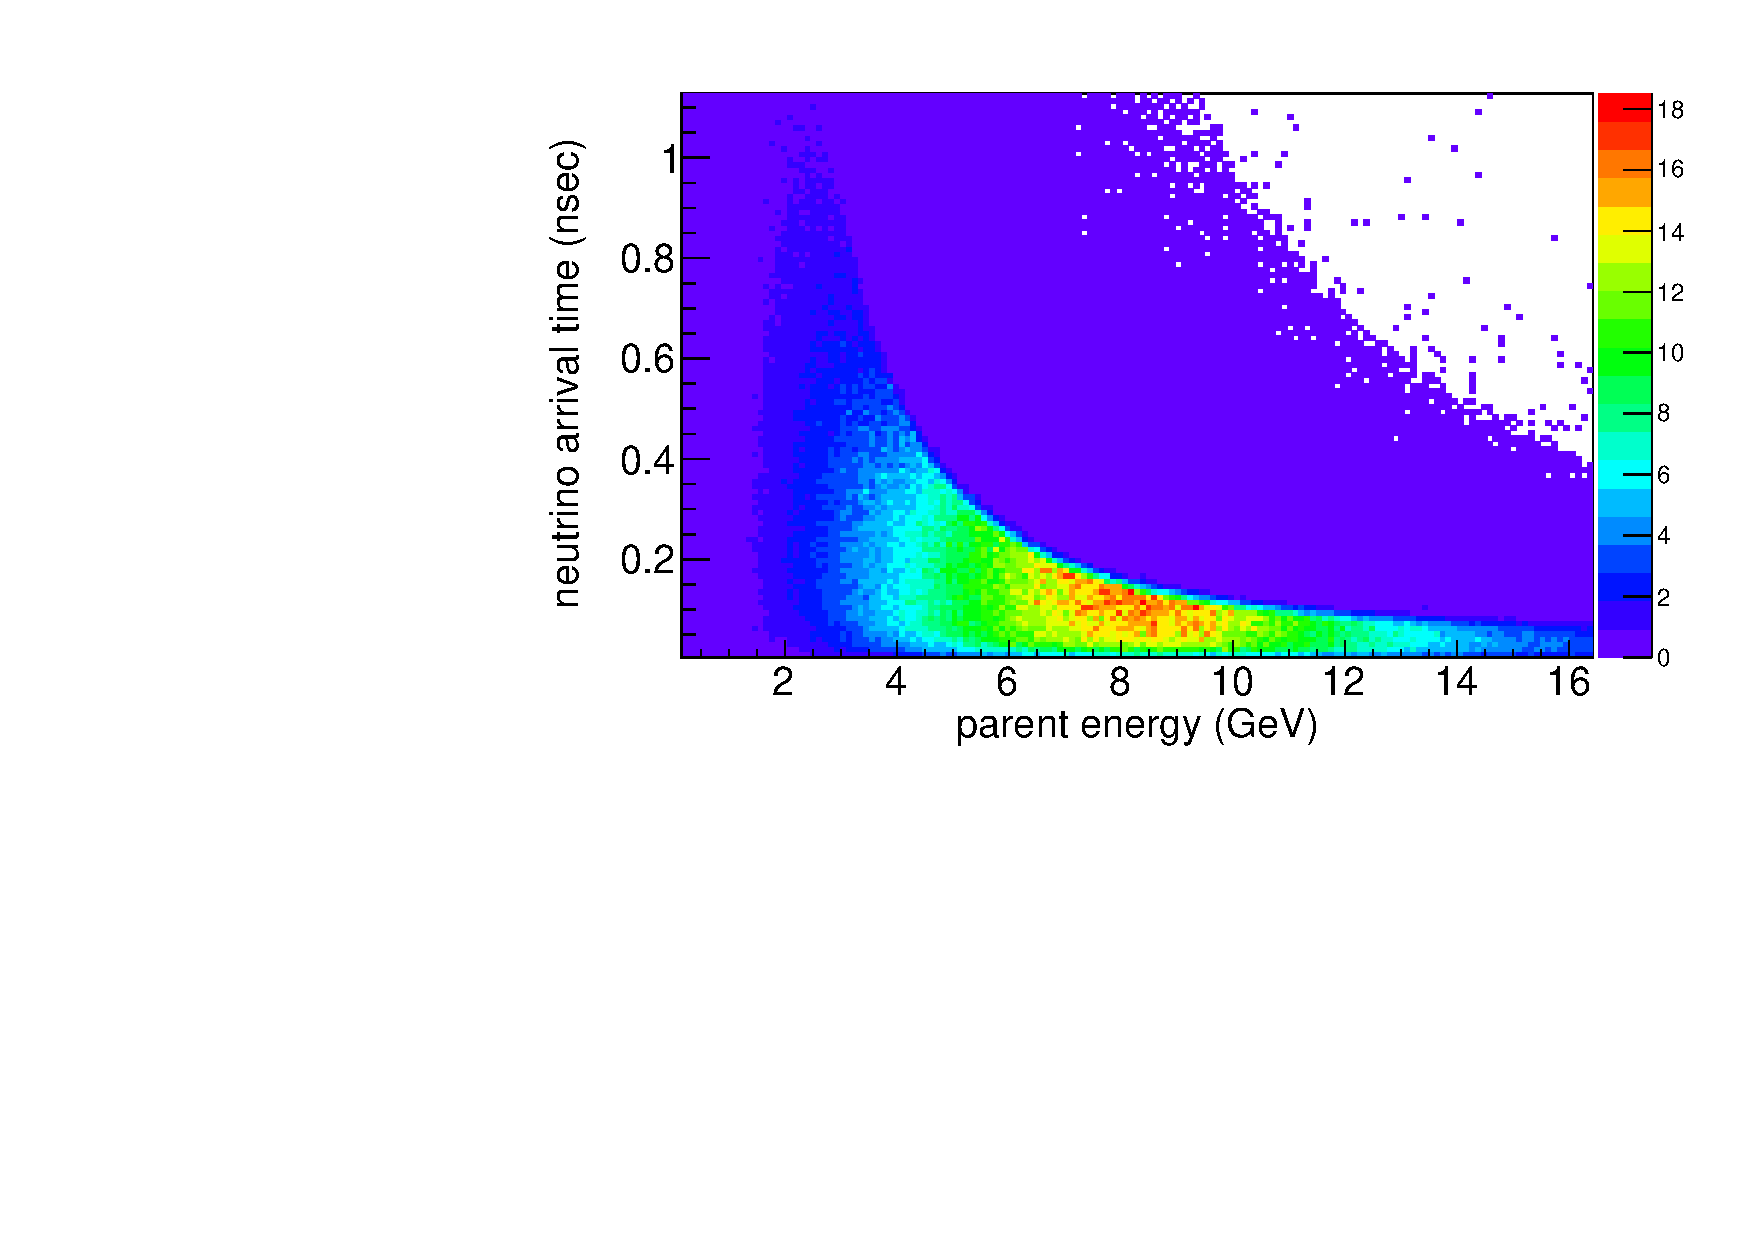
\includegraphics[width=0.45 \linewidth]{Figures/14.10.18_LBNFtiming/parentEvsdT.pdf} &
			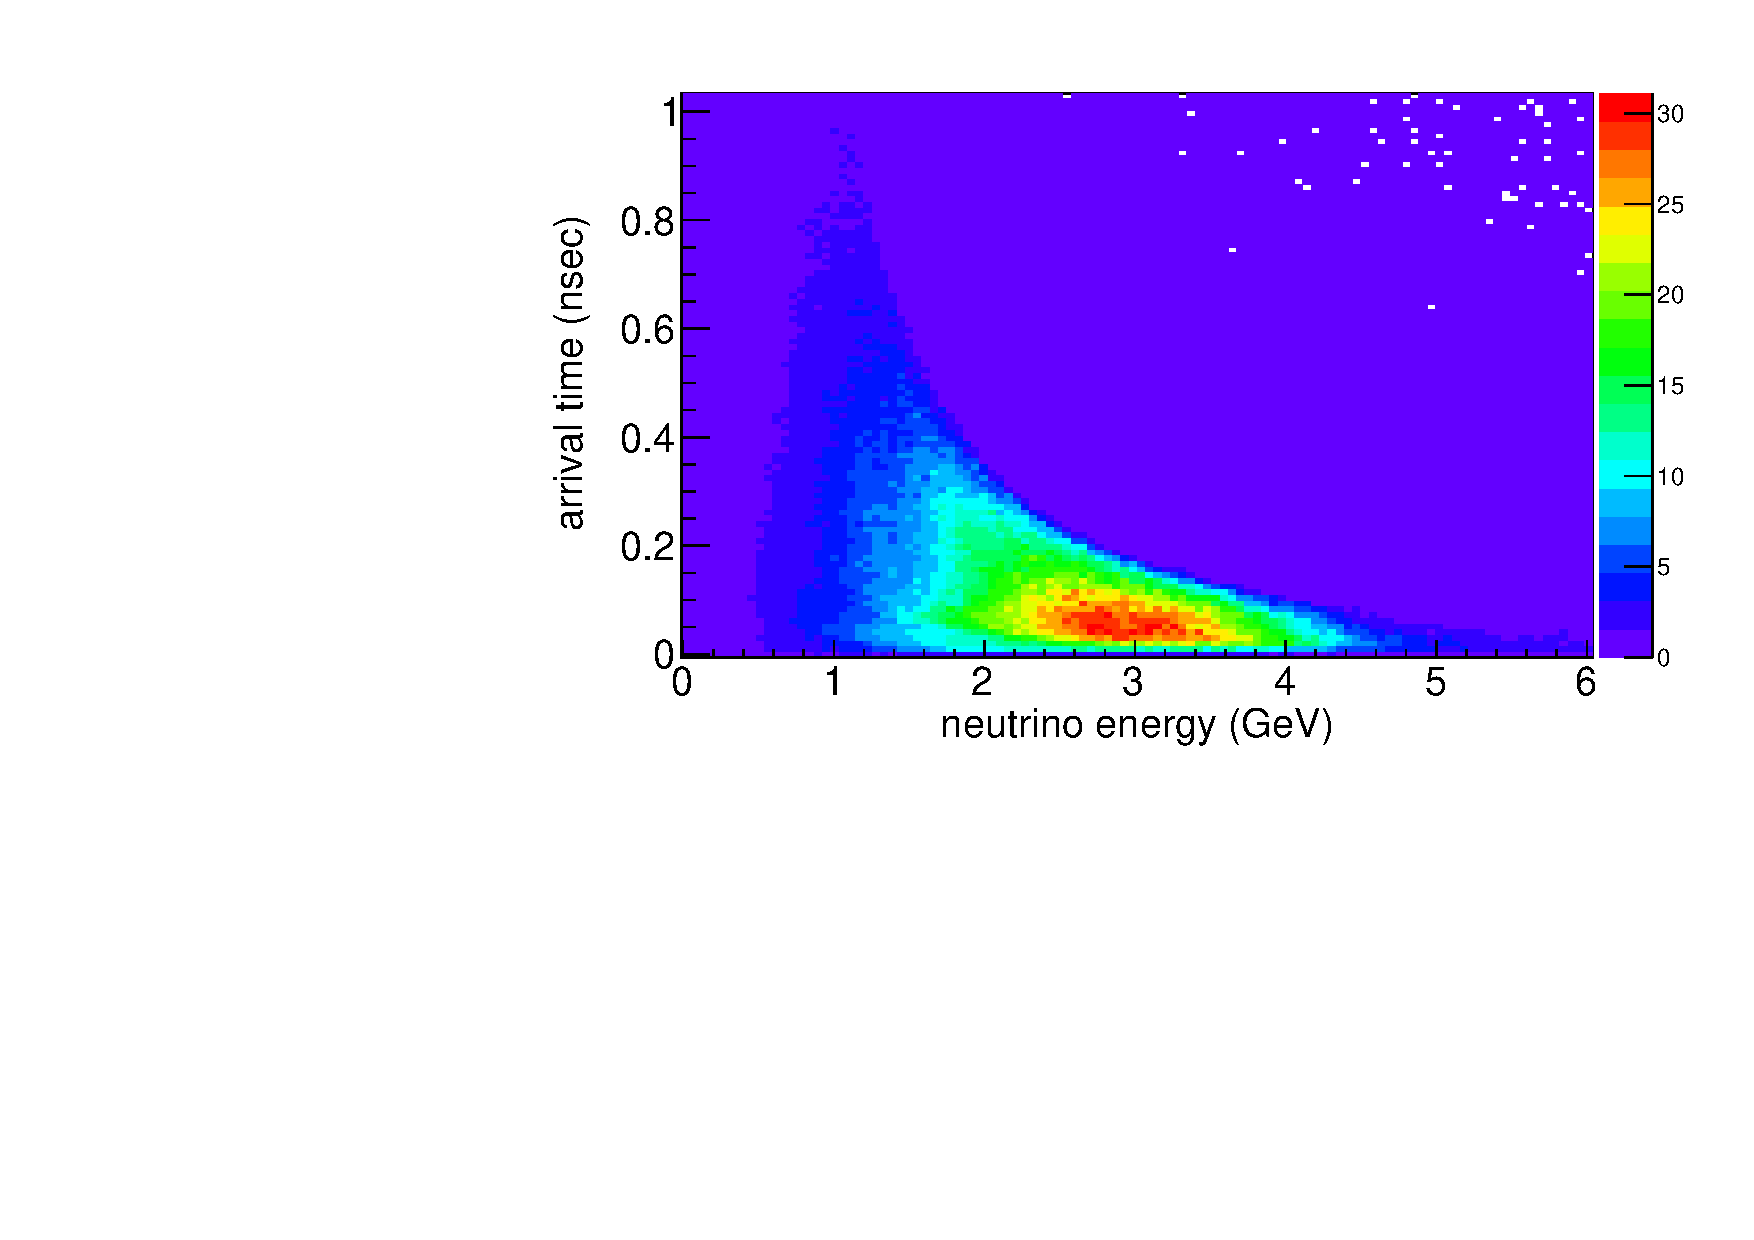
\includegraphics[width=0.45 \linewidth]{Figures/14.10.18_LBNFtiming/nuEvsdT.pdf} \\
			\end{tabular}
	\end{center}
	\caption{LEFT: The relationship between the arrival times and pion energies, for a population of pions produced at the same time. RIGHT: ..}
		\label{fig:anniedetector}
\end{figure}


\section{Physics Case}

The impact of energy uncertainty on precision oscillation measurements. How slices in energy spectra can control that systematic. The impact on oscillation physics. Connection to Theia and second maximum. Other impacts.


\section{Impact of Bunch Size on the Effect}

Just showing that wider bunches wash out the effect (short section)

\begin{figure}[t]
	\begin{center}
           	\begin{tabular}{c c}	
           	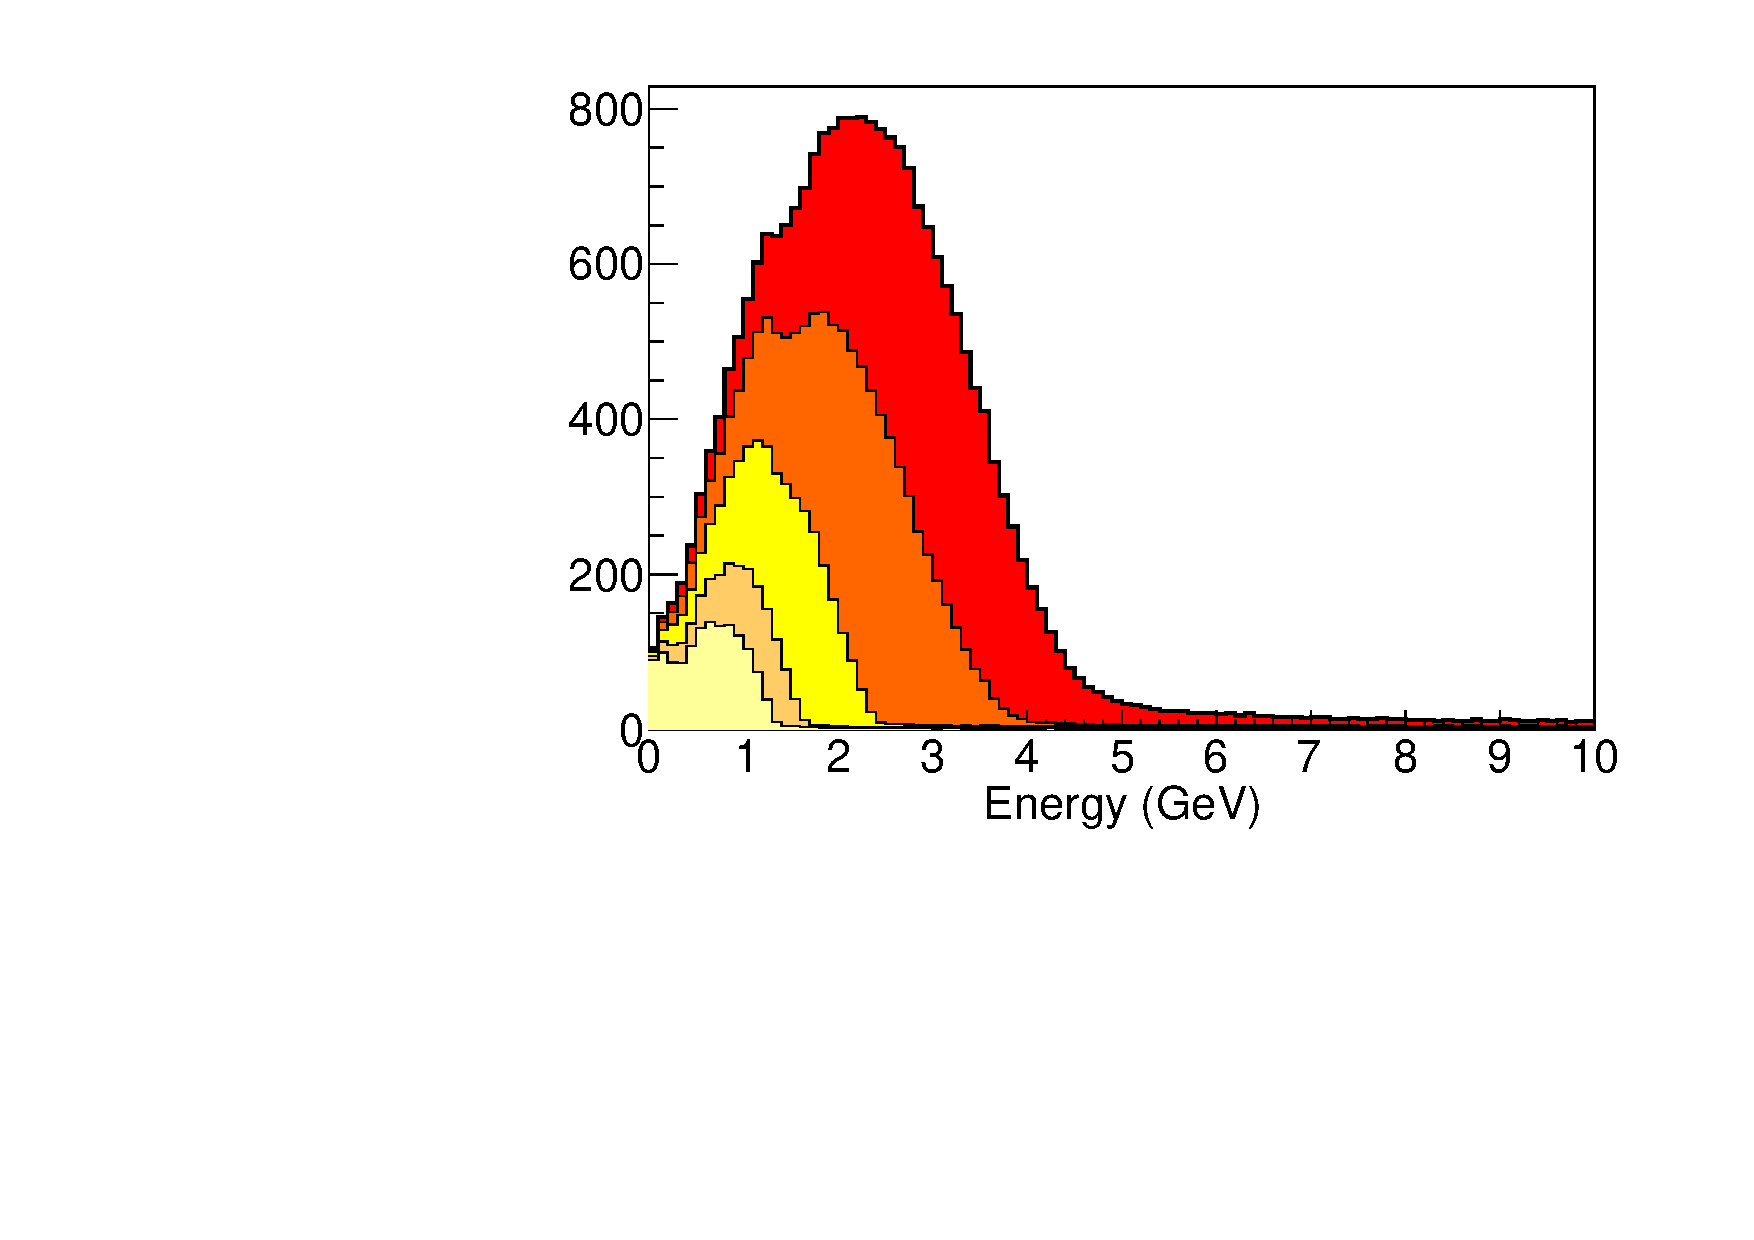
\includegraphics[width=0.45 \linewidth]{Figures/10.10.18_LBNFtiming/DUNEbeam_truetimingB.pdf} &
			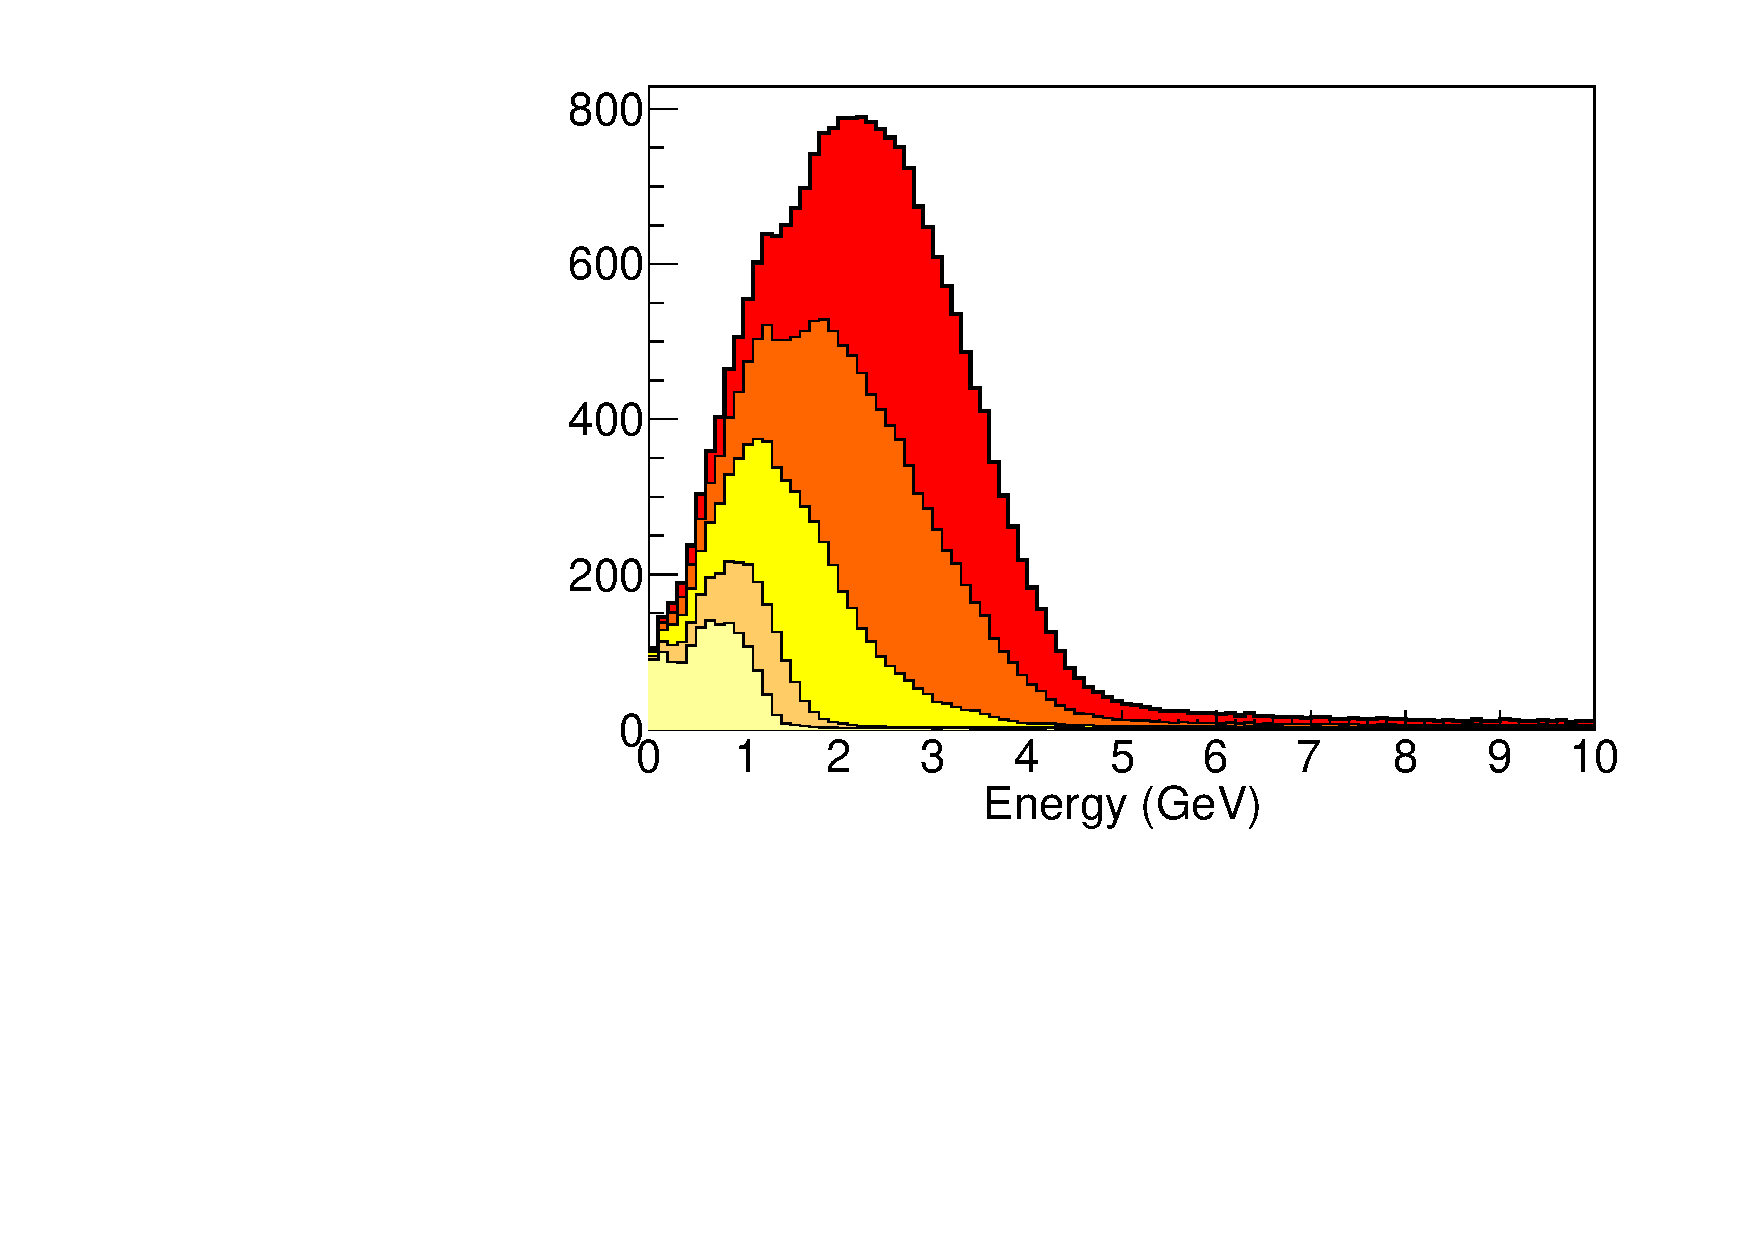
\includegraphics[width=0.45 \linewidth]{Figures/10.10.18_LBNFtiming/DUNEbeam_100psecB.pdf} \\
           	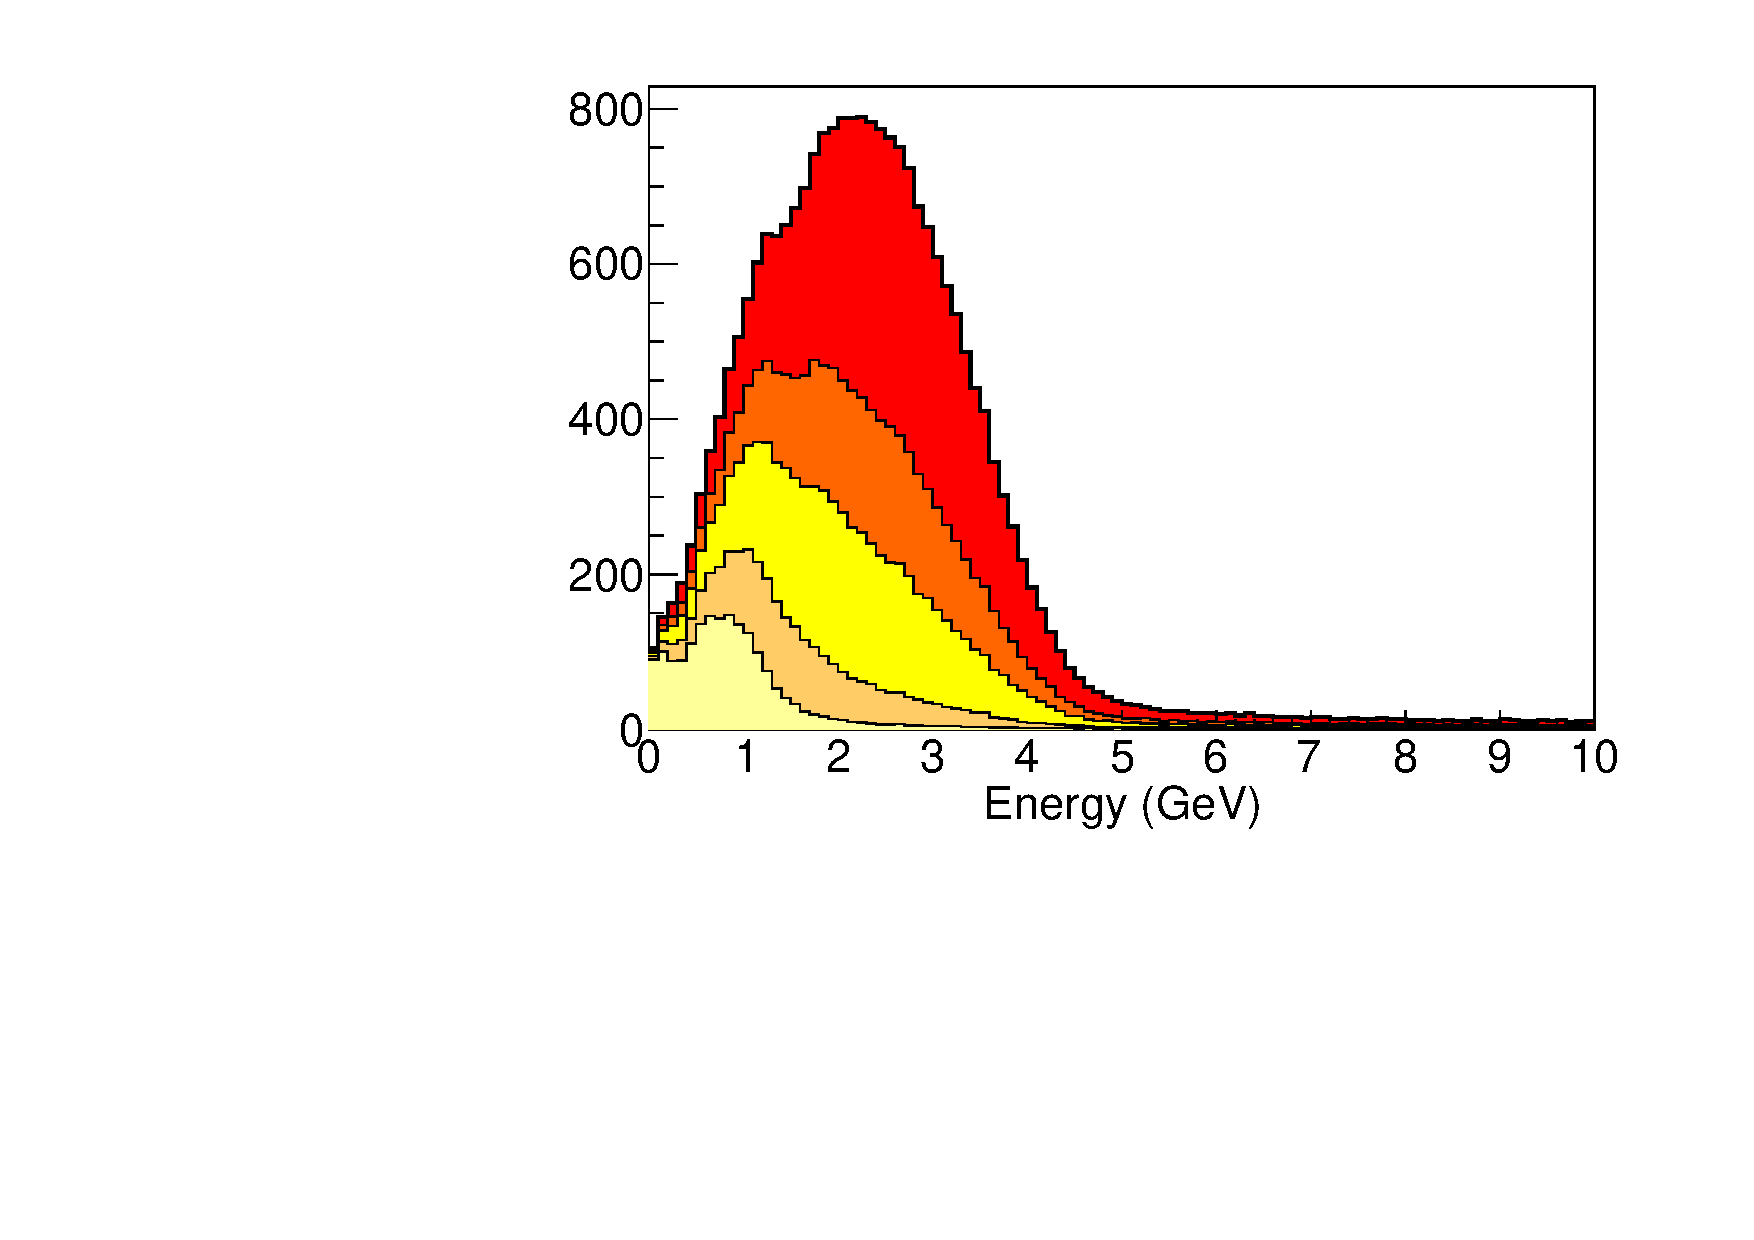
\includegraphics[width=0.45 \linewidth]{Figures/10.10.18_LBNFtiming/DUNEbeam_250psecB.pdf} &
			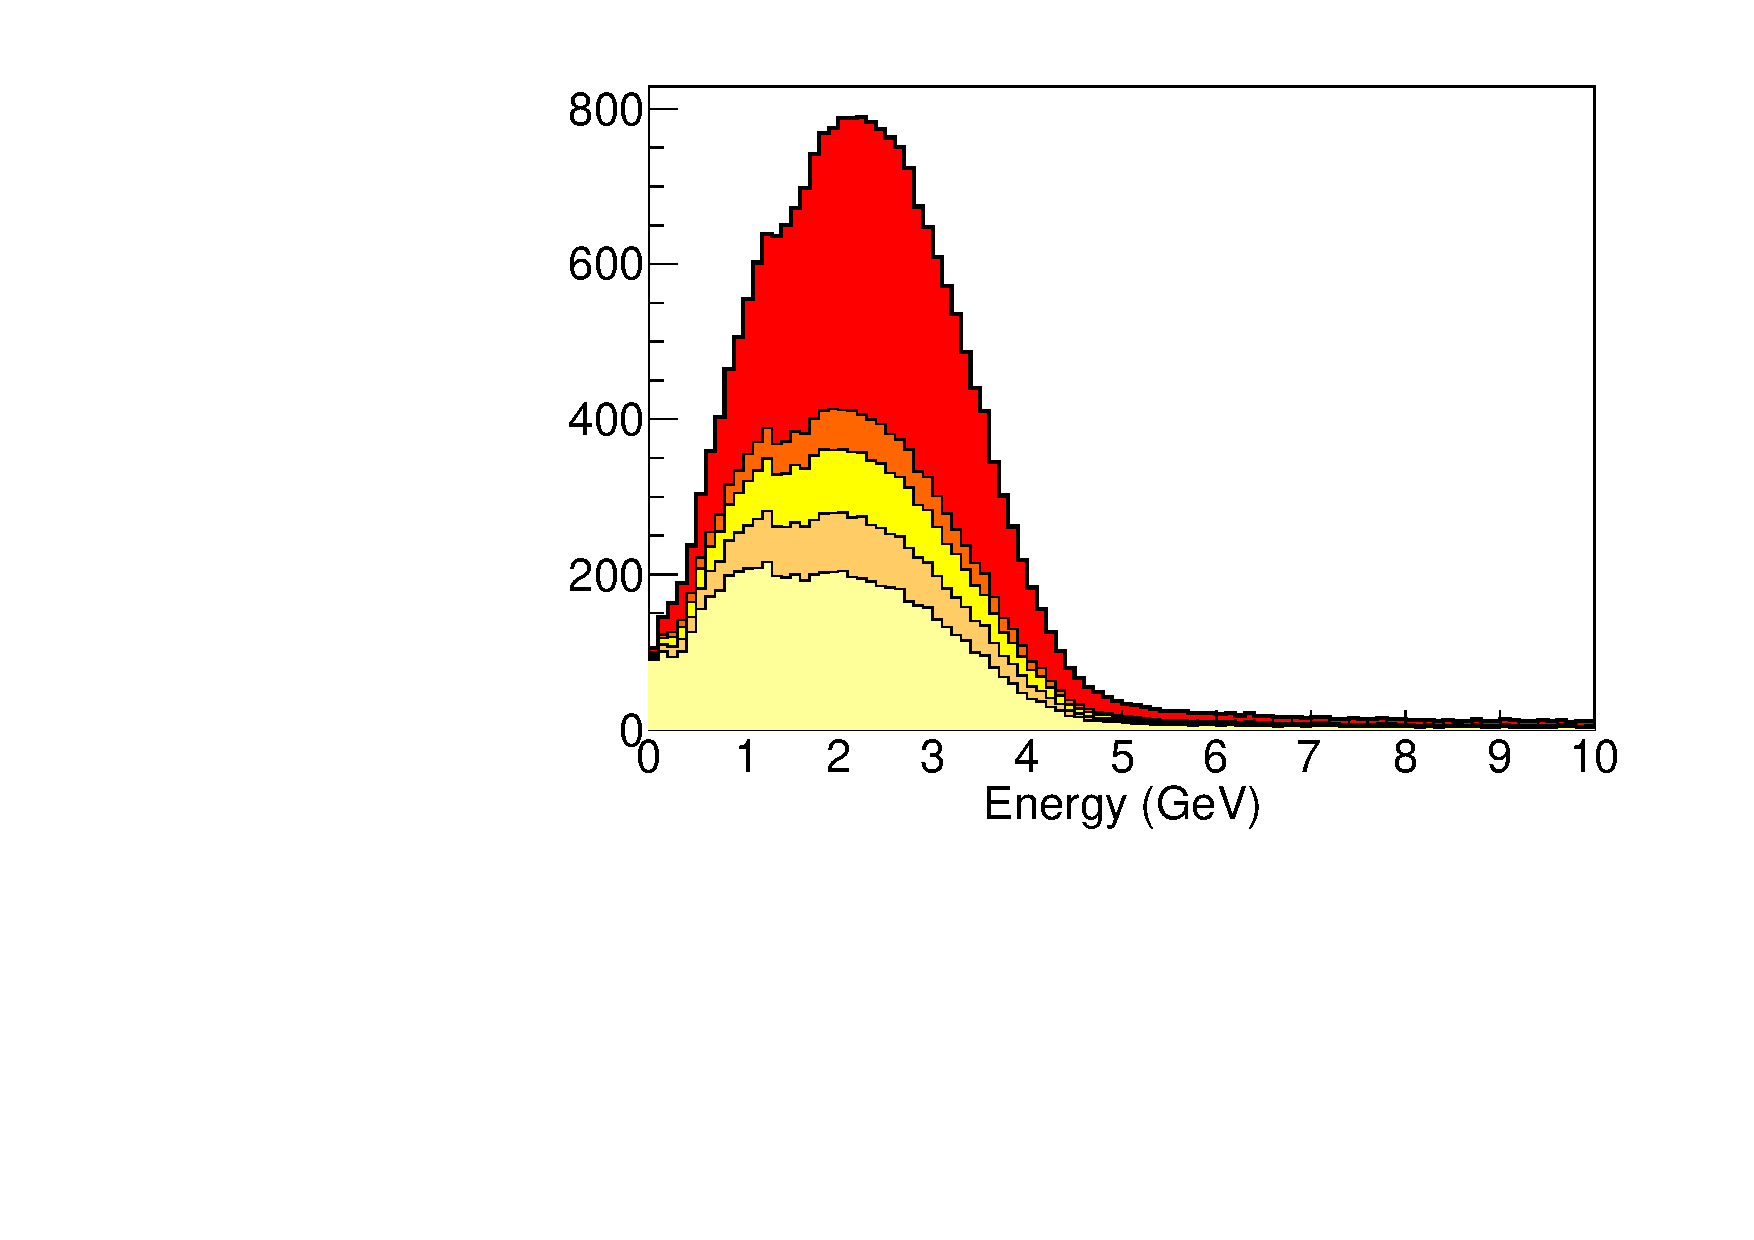
\includegraphics[width=0.45 \linewidth]{Figures/10.10.18_LBNFtiming/DUNEbeam_900psecB.pdf}
			 \\			
			\end{tabular}
	\end{center}
	\caption{LEFT: The relationship between the arrival times and pion energies, for a population of pions produced at the same time. RIGHT: ..}
		\label{fig:anniedetector}
\end{figure}


\section{Superimposing a Fine Bunch Structure at 500 MHz: Concept and Feasibility}

Talking about how this could be done, how big a change it would be, how hard, etc

\section{Achieving 100 psec Trigger Resolution}

Jonathan Eisch - getting beam information, making fast triggers, etc

\section{Achieving 100 psec Vertex Resolution}


\section{Conclusion}

This is great.

%% The Appendices part is started with the command \appendix;
%% appendix sections are then done as normal sections
%% \appendix

%% \section{}
%% \label{}

%% References
%%
%% Following citation commands can be used in the body text:
%% Usage of \cite is as follows:
%%   \cite{key}          ==>>  [#]
%%   \cite[chap. 2]{key} ==>>  [#, chap. 2]
%%   \citet{key}         ==>>  Author [#]

%% References with bibTeX database:

\bibliographystyle{model1-num-names}
\bibliography{bibliography.bib}

%% Authors are advised to submit their bibtex database files. They are
%% requested to list a bibtex style file in the manuscript if they do
%% not want to use model1-num-names.bst.

%% References without bibTeX database:

% \begin{thebibliography}{00}

%% \bibitem must have the following form:
%%   \bibitem{key}...
%%

% \bibitem{}

% \end{thebibliography}


\end{document}

%%
%% End of file `elsarticle-template-1-num.tex'.